\section{Methodological and Theoretical Framework}
\subsection{Cognitive Sovereignty and Thermodynamics: Definition and Implications}

From the thermodynamic analysis and archaeological evidence emerges a pattern of architectural transformation: the systematic collapse of sphere-like cognitive structures into vector-like configurations.

We employ thermodynamic analysis not for complexity but for clarity. Thermodynamics is simply the science of why things require energy to maintain their organization. Your house requires cleaning, your car requires maintenance, your body requires food. This is all because the Second Law of Thermodynamics states that organized systems naturally decay toward disorder unless energy is invested to maintain them. Knowledge is no different: without the energy investment of practice, study, and application, expertise degrades to rote memorization and eventually to what Feynman termed 'Cargo Cult Science', the empty mimicry of expertise without understanding \citep{feynman1974}. That this term has become ubiquitous in organizational development literature, from diagnosing 'cargo cult analytics' \citep{mcnamee2019} to identifying hollow institutional practices \citep{alvesson2013}, reveals an uncomfortable truth: these thermodynamically depleted rituals have become the norm rather than the exception. We perform the motions of knowledge work without possessing its substance. When we speak of 'thermodynamic collapse,' we mean the predictable result of trying to maintain complex systems (like human expertise) without investing the energy they require. It is like expecting a garden to thrive without water, sunlight, or care.

A sphere represents multidimensional cognitive architecture: extensive cross-domain connections, adaptive capacity across contexts, emergent synthesis from diverse knowledge. Topologically, it exhibits high connectivity density, multiple paths between concepts, resilience through redundancy. Thermodynamically, it represents high negentropy requiring sustained energy investment across many domains simultaneously.

A vector represents unidimensional optimization: specialized expertise in narrow channels, efficiency in known contexts, predetermined responses. Topologically, it exhibits linear structure, minimal cross-connections, brittleness through specialization. Thermodynamically, it represents lower local negentropy concentrated in specific dimensions, requiring less sustained investment but offering less adaptability.

These are not mere metaphors but measurable architectures. Network analysis can map conceptual connectivity. Performance metrics can assess adaptation versus optimization. Energy investment can be tracked in time allocation across domains. The sphere-to-vector transformation appears in observable changes: declining breadth of study, increasing specialization, reduced cross-domain practice.

\subsubsection{The Thermodynamic Equation}

The energy investment equation crystallizes this relationship with physical precision:

\begin{equation}
\text{Cognitive Sovereignty [W]} = \frac{\text{Energy Invested [J]}}{\text{Time [s]}} \times \text{Resistance to Extraction [0-1]}
\end{equation}

Where: Energy Investment Rate $>$ Entropy Rate

This formulation grounds abstract concepts of knowledge and expertise in fundamental physics, using the same units (Watts) that Vaclav Smil employs to trace energy transitions from agricultural societies ($10^4$ W/capita) through industrial ($10^5$ W/capita) to modern technological civilization ($10^6$ W/capita) \citep{smil2017}. Just as Smil demonstrates that civilizational complexity requires specific power densities, cognitive complexity requires specific power investments above the brain's baseline consumption of approximately 20 Watts \citep{raichle2002}.

The marginal watt of active cognition (approximately 5\% above baseline \citep{jamadar2025}) determines whether an individual operates as a sovereign cognitive agent or merely processes predetermined patterns. This distinction becomes critical when scaled to civilizational level, where the proportion of population engaged in knowledge work multiplies this marginal investment.

\subsubsection{Components and Measurement}

The equation's elegance emerges from its two multiplicative components:

\textbf{Power Component (E/t):} Quantifies the rate of energy investment in cognitive development. Historical analysis reveals exponential decay in investment intensity:

\begin{itemize}
\item Ancient Greek philosophical education: 20 years $\times$ 2000 hours/year = 144 MJ total
\item Medieval guild apprenticeship: 7 years $\times$ 2500 hours/year = 63 MJ
\item Contemporary bachelor's degree: 3 years $\times$ 1000 hours/year = 10.8 MJ
\item Modern micro-credential: 40 hours = 0.144 MJ
\end{itemize}

This thousand-fold reduction in energy investment parallels what Smil identifies as ``efficiency paradoxes'' where increased efficiency reduces system resilience \citep{smil2018}.

\textbf{Resistance Component (R):} To be unambiguous: \textbf{R (extraction resistance) IS architectural quality, not a correlate or proxy.} High-quality cognitive architecture manifests AS resistance to algorithmic extraction. Low-quality architecture manifests AS ease of proceduralization. The R value doesn't measure something adjacent to quality; it operationally defines what quality means in thermodynamic terms.

\begin{table}[h]
\centering
\caption{R as Architectural Quality Across Descriptive Frameworks}
\begin{tabular}{|c|c|l|l|l|l|}
\hline
\textbf{R} & \textbf{Range} & \textbf{Geometry} & \textbf{Cynefin} & \textbf{Anthropologic} & \textbf{Silicon Status} \\
\hline
1.0 & 1.0 & Hypersphere & --- & Theoretical maximum & --- \\
0.7 & 0.7-0.9 & Sphere & Chaotic & Renaissance polymath & --- \\
0.4 & 0.4-0.7 & Ellipsoid & Complex & Complex domain navigator & --- \\
0.2 & 0.2-0.4 & Cylinder & Complicated & Complicated domain specialist & GPT-5.x ceiling \\
0.1 & 0.0-0.2 & Vector & Clear & Procedural executor & Current LLMs \\
0.0 & 0.0 & Point & --- & Pure algorithm & --- \\
\hline
\end{tabular}
\end{table}

\textit{Note: These are theoretical positions based on documented characteristics, not empirical measurements. We DEFINE a Renaissance polymath as exhibiting R $\approx$ 0.7-0.9 based on their demonstrated capacity for cross-domain synthesis that resisted standardization for centuries. We POSITION current LLMs at R $\approx$ 0.1-0.2 based on their observable performance in procedural versus emergent domains.}

We propose multiple measurement approaches, recognizing contextual specificity:

\begin{enumerate}
\item \textbf{Dimensional Diversity} ($R_1$): $R = 1 - (1/n)$, where $n$ represents integrated knowledge domains
\item \textbf{Network Density} ($R_2$): Ratio of actual to possible conceptual connections
\item \textbf{Information Complexity} ($R_3$): Kolmogorov incompressibility measure
\item \textbf{Cynefin Classification} ($R_4$): Domain-specific resistance \{Clear: 0.1, Complicated: 0.3, Complex: 0.7, Chaotic: 0.9\}
\item \textbf{Knowledge Portfolio} ($R_5$): Active knowledge types relative to historical maximum
\end{enumerate}

Practitioners may employ individual metrics or weighted combinations ($R = \sum w_i \times R_i$) appropriate to their specific context. Critically, resistance exhibits temporal decay without maintenance: $R(t) = R_0 \times e^{-\lambda t}$, where $\lambda$ varies by knowledge type from 0.05/year for embodied skills to 1/year for micro-credentials.

\subsubsection{Civilizational Implications}

Scaling from individual to civilizational level reveals profound implications. The total cognitive power available to civilization equals:

\begin{equation}
\text{Civilizational Cognitive Power} = \text{Population} \times \text{Knowledge Worker Fraction} \times 21\text{W} \times \bar{R}
\end{equation}

Where $\bar{R}$ represents population-weighted average resistance. Historical trajectory analysis yields concerning patterns:

\begin{table}[h]
\centering
\caption{Civilizational cognitive power trajectory (*projected values based on observed decay acceleration)}
\begin{tabular}{|l|r|r|r|r|r|r|}
\hline
Era & Population & Knowledge & Cognitive & $\bar{R}$ & Effective & Efficiency \\
    &            & Workers   & Budget    &           & Power     &            \\
\hline
1800 & 1B & 1\% & 210 MW & 0.80 & 168 MW & 80\% \\
1950 & 2.5B & 10\% & 5.25 GW & 0.50 & 2.6 GW & 50\% \\
2024 & 8B & 40\% & 67.2 GW & 0.10 & 6.7 GW & 10\% \\
2040* & 9B & 50\% & 94.5 GW & 0.04* & 3.8 GW* & 4\%* \\
2060* & 10B & 60\% & 126 GW & 0.008* & 1.0 GW* & $<$1\%* \\
\hline
\end{tabular}
\end{table}

%% FIGURE MARKER: Insert Figure 2 - Knowledge Worker Paradox
\begin{figure}[h]
\centering
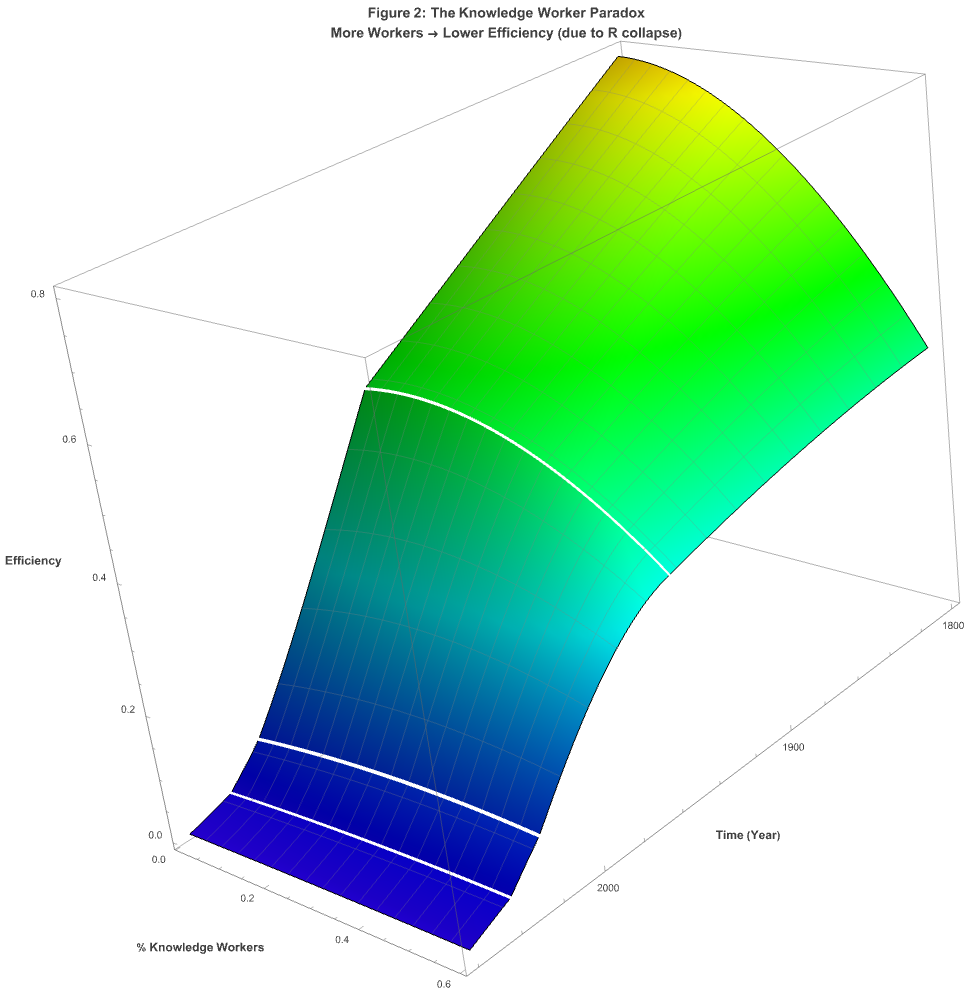
\includegraphics[width=0.85\textwidth]{knowledge_worker_paradox}
\caption{The Knowledge Worker Paradox: More workers correlates with lower efficiency due to R collapse}
\label{fig:knowledge_worker_paradox}
\end{figure}

%% FIGURE MARKER: Insert Figure 3 - Effective Cognitive Power
\begin{figure}[h]
\centering
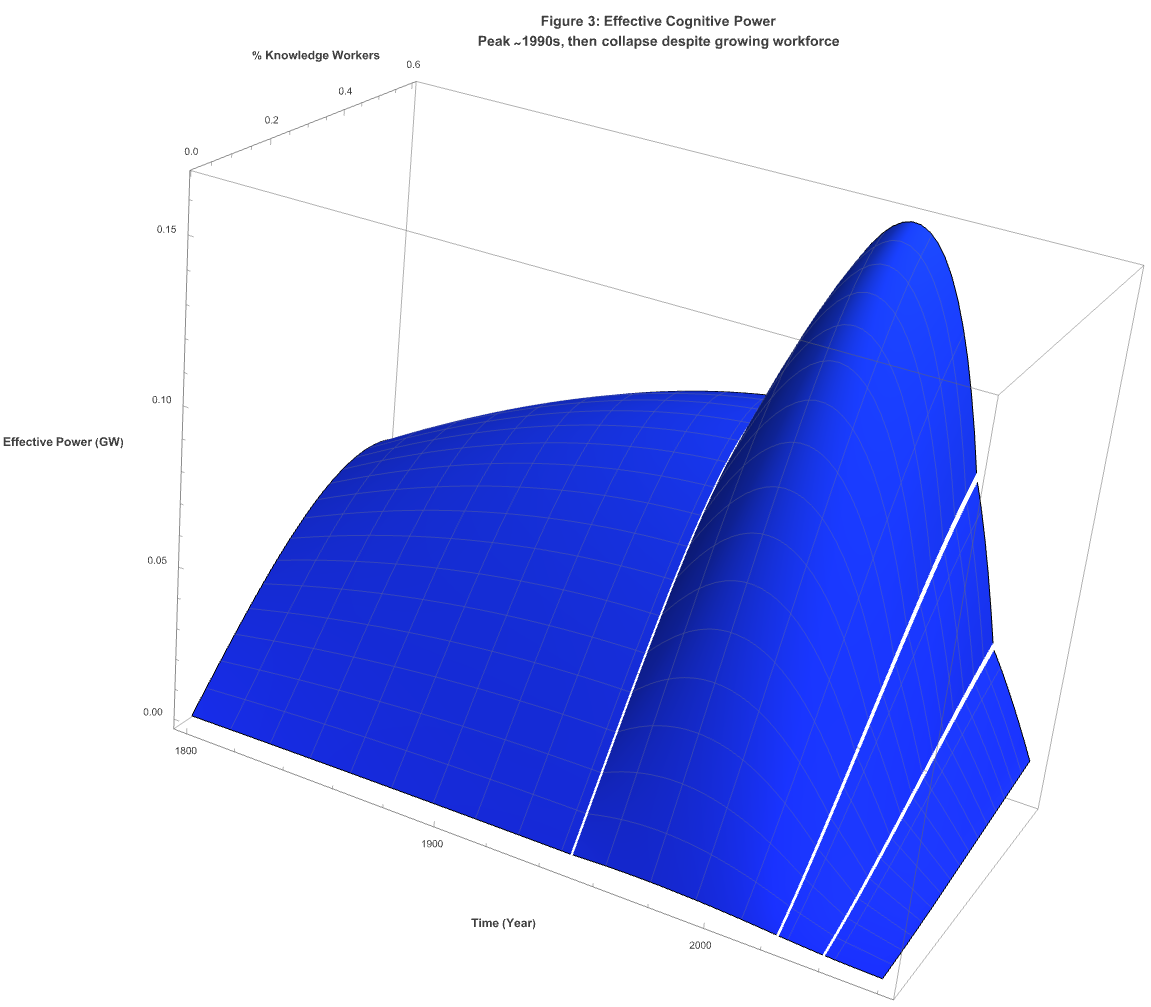
\includegraphics[width=0.85\textwidth]{effective_cognitive_power}
\caption{Effective Cognitive Power: Despite a 320-fold increase in knowledge workers, effective power peaks around 1980 then collapses}
\label{fig:effective_cognitive_power}
\end{figure}

%% FIGURE MARKER: Insert Figure 4 - Resistance to Extraction Collapse
\begin{figure}[h]
\centering
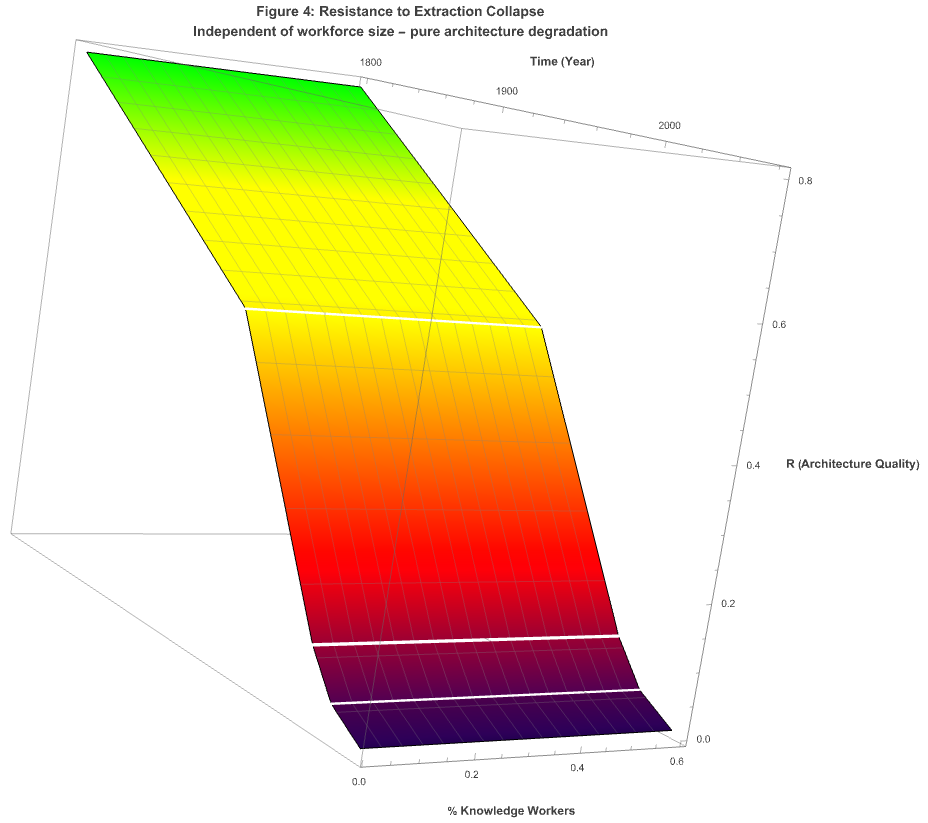
\includegraphics[width=0.85\textwidth]{resistance_collapse}
\caption{Resistance to Extraction Collapse: The architectural transformation from sphere (R $\approx$ 0.8) to vector (R $\approx$ 0.1) visualized across 200+ years}
\label{fig:resistance_collapse}
\end{figure}

%% FIGURE MARKER: Insert Figure 2d - Efficiency per Knowledge Worker
\begin{figure}[h]
\centering
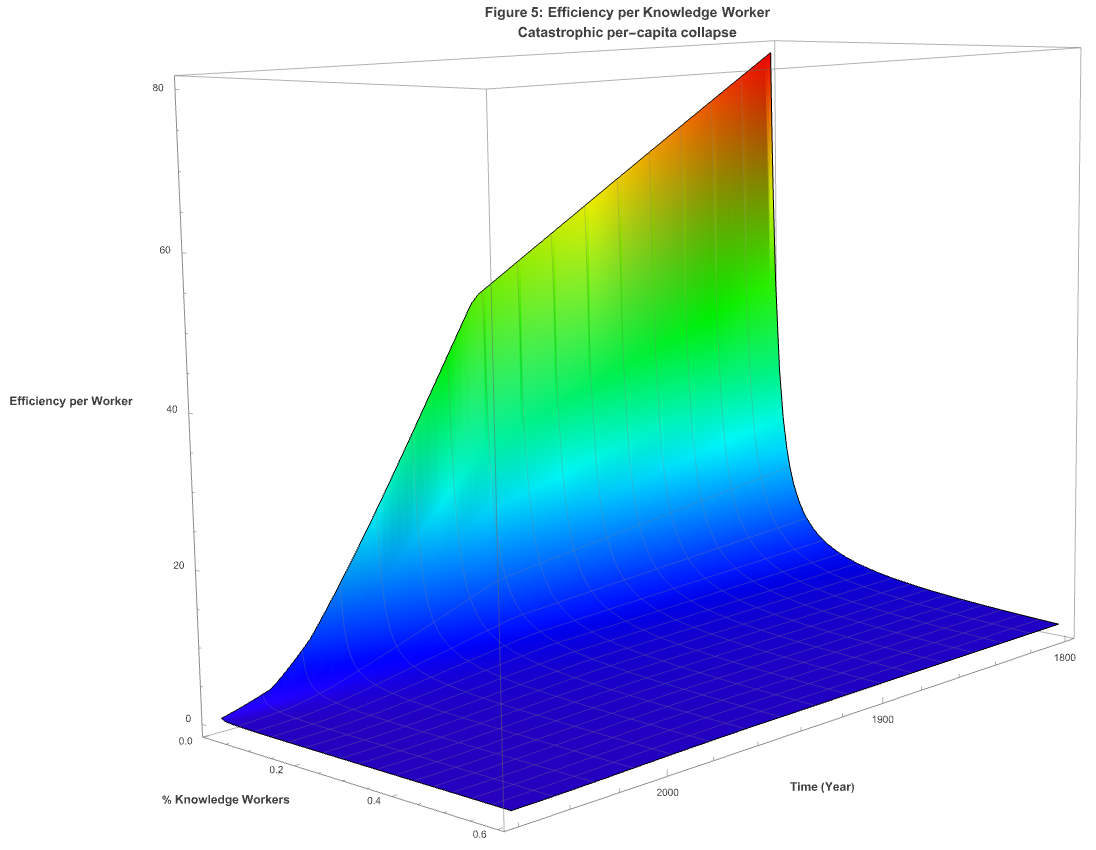
\includegraphics[width=0.85\textwidth]{efficiency_collapse}
\caption{Efficiency per Knowledge Worker: Catastrophic per-capita collapse from 80\% to near-zero}
\label{fig:efficiency_collapse}
\end{figure}

%% FIGURE MARKER: Insert Figure 2e - Convergent Collapse Validation
\begin{figure}[h]
\centering
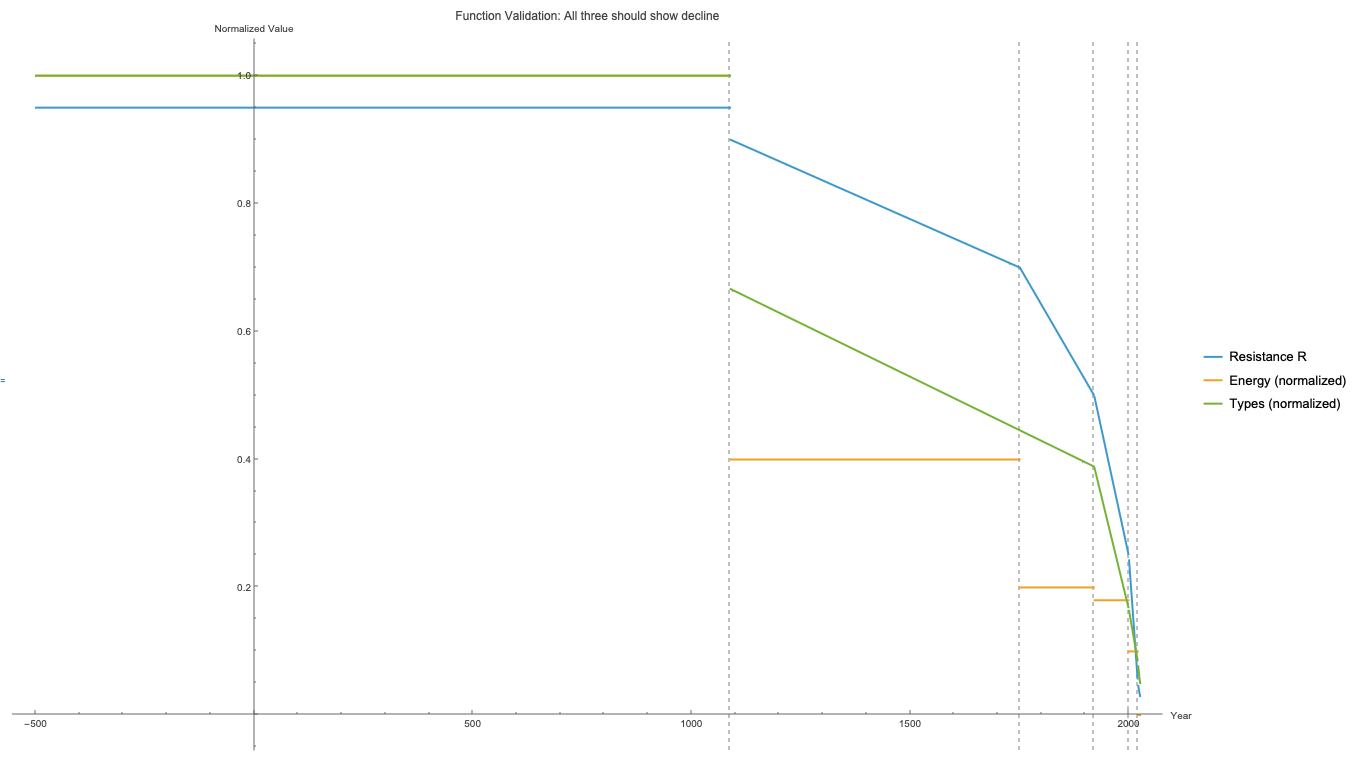
\includegraphics[width=0.85\textwidth]{convergent_validation}
\caption{Convergent Collapse Validation: Three independent measures show identical patterns}
\label{fig:convergent_validation}
\end{figure}

The visualizations demonstrate what Smil calls ``the paradox of efficiency'': as we optimize for more knowledge workers at lower training costs, total effective cognitive power collapses despite increased nominal capacity.

The data reveal that despite a 320-fold increase in cognitive energy expenditure since 1800, effective sovereignty has increased only 40-fold: a negative return to scale that violates fundamental principles of sustainable systems \citep{smil2019}. The observed decay in $\bar{R}$ from 0.002/year (1800-1950) to 0.0054/year (1950-2024) suggests acceleration rather than stabilization.

\subsubsection{Operational Applications}

The framework enables precise interventions across scales:

\textbf{Individual Level:} Professionals can calculate and optimize their Cognitive Sovereignty through deliberate practice scheduling \citep{ericsson1993}, dimensional diversity cultivation, and decay monitoring. Target maintenance: $>$1W effective sovereignty (2W investment $\times$ 0.5 resistance minimum).

\textbf{Organizational Level:} Institutions can map cognitive power distribution, identify extraction vulnerabilities, and design appropriate ``cognitive infrastructure'' with specific decay constants. German engineering education's resistance to modularization, maintaining five-year integrated programs despite Bologna pressure, exemplifies successful sovereignty preservation.

\textbf{Societal Level:} The equation quantifies why educational ``efficiency'' destroys capability. Bologna Process reforms reduced both E/t (by 60\%) and R (by 70\%), yielding 88\% sovereignty loss, precisely matching observed digital transformation failure rates \citep{bain2024}.

\subsubsection{Validation Through Convergent Evidence}

These theoretical positions gain validity through multiple convergent indicators:

\textbf{Historical Documentation:} Renaissance polymaths required 20+ years of comprehensive education across philosophy, mathematics, arts, and sciences. Contemporary micro-credentials require hours to days. The energy investment ratio of 10,000:1 maps directly to the R differential.

\textbf{Performance Evidence:} LLMs excel at tasks requiring R $<$ 0.2 (code completion, translation, summarization) but systematically fail at tasks requiring R $>$ 0.4 (paradigm creation, contextual ethics, novel framework development). The 42\% AI project abandonment rate occurs precisely when organizations attempt to deploy low-R systems for high-R challenges.

\textbf{Architectural Isomorphism:} Transformer architectures literally implement vector processing through tokenization (fragmentation), embedding (standardization), and attention (selective focus). They are mathematically constrained to R $<$ 0.3 by their architectural foundations.

\textbf{Measurement Convergence:} Five independent approaches yield consistent R classifications, suggesting R captures a fundamental property rather than arbitrary categorization.

\subsubsection{Thermodynamic Constraints and Trajectories}

The framework reveals inescapable thermodynamic constraints. Current trajectories, if maintained, project continued decay of civilizational cognitive sovereignty. The intersection of increasing population, rising knowledge worker percentage, and declining resistance creates what systems theorists recognize as a ``competency trap'' \citep{levitt1988}: apparent success masking fundamental deterioration.

The critical threshold occurs when $\bar{R}$ falls below approximately 0.05, at which point complex civilization becomes unsustainable according to Tainter's complexity collapse model \citep{tainter1988}. Current decay rates suggest this threshold approaches within decades rather than centuries. Unlike climate change, which operates on geological timescales with debated tipping points, cognitive sovereignty decay follows exponential curves with mathematically determinable inflection points.

The implications extend beyond workforce concerns. As Smil demonstrates \citep{smil2017}, every civilizational transition required order-of-magnitude increases in power density. We face an inverse transition: maintaining information-age complexity while experiencing order-of-magnitude decreases in cognitive power density. This violates fundamental thermodynamic principles: no complex system can maintain organization while reducing energy throughput below critical thresholds.

\subsubsection{Reconstruction Possibilities}

The equation also identifies reconstruction pathways. Reversing cognitive decline requires either increasing power investment (E/t) or architectural complexity (R), ideally both. Historical precedents exist: the Renaissance recovered from medieval vectorization through massive reinvestment in multidimensional education. The German engineering resistance demonstrates contemporary possibility.

However, the window for intervention narrows. The cohort experiencing pre-Bologna education ages out by 2040-2050, taking embodied knowledge of sphere development with them. Without deliberate preservation and transmission, reconstruction becomes archaeological rather than pedagogical: attempting to reverse-engineer what we deliberately destroyed.

The choice facing individuals and institutions is thus genuinely binary: invest the energy required for cognitive sovereignty or accept thermodynamic dissolution into extractive systems. Physics, as we note throughout this analysis, doesn't negotiate.